\section{Evaluation}
\label{sec:evaluation}

The evaluation asks four questions of the deployment: does an
LLM alone suffice for CompOps operator questions? Does a RAG
pipeline over the documented corpus suffice? Does the agent
loop earn its keep over single-shot RAG? Do live MonIT tool
calls earn their cost over a doc-only agent?
Section~\ref{sec:eval_methodology} states the configurations,
models, and infrastructure for the two experimental tracks
(260-question single-judge matrix on local Ollama, 53-question
multi-judge subset on OpenRouter).
Section~\ref{sec:eval_lifts} walks the four-step lift from a
bare LLM (\textbf{2.86}) to the full agent (\textbf{4.22})
under \texttt{glm-5.1} on the 260-question set.
Section~\ref{sec:eval_costs} surfaces the two costs the agent
loop carries.
Section~\ref{sec:eval_ensemble} replicates the ordering under a
four-judge ensemble on a 53-question subset.
Section~\ref{sec:eval_human_53} reports the human evaluation
panel.

\subsection{Configurations, models, and infrastructure}
\label{sec:eval_methodology}

Two experimental tracks share the same rubric and pipeline
definitions but differ in scale, judge protocol, and model
selection.

\paragraph{260-question matrix on local Ollama.}
The four pipelines of Section~\ref{sec:pipelines} (the bare-LLM
control, the RAG control, the agent without live operational
tools, and the agent) run on three locally-served open-weight
models: \texttt{gemma4-26b}~\cite{gemma4card}, a Google
mixture-of-experts (MoE) with 26\,B total and 4\,B active
parameters; \texttt{qwen3.5-27b}~\cite{qwen3report}, a 27\,B
dense model from Alibaba; and
\texttt{qwen3.5-122b-a10b}~\cite{qwen3report}, a 122\,B MoE
with 10\,B active per token. Each (pipeline, model) combination
runs with the model's extended-thinking mode (the model emits a
chain-of-thought trace before its answer) enabled and,
separately, disabled. All models in this track are served
through Ollama~\cite{ollama} on a CMS-internal node with four
NVIDIA Tesla V100-SXM2-32GB GPUs (128\,GB total VRAM, NVLink).
The reference column is the 237 production answers generated
by the deployed GPT-5.3 pipeline (23 of 260 questions, drawn
from \texttt{jira\_investigation} and \texttt{debugging}, were
not answered during the recorded session); these answers are
scored alongside the open-weight pipelines under the same judge
and rubric.

\paragraph{53-question subset on OpenRouter.}
A five-configuration subset addresses the agent-vs-RAG and
frontier-vs-open-weight comparisons that fall outside the local
cluster's VRAM and model availability: the closed-frontier
\texttt{gpt-5.5-2026-04-23} agent with live tools (a more
recent OpenAI release than the deployed GPT-5.3), the
\texttt{qwen3.5-122b-a10b} agent (shared with the 260q track),
the \texttt{qwen3.6-35b-a3b} agent, the \texttt{qwen3.6-27b}
agent, and a \texttt{qwen3.6-27b} single-shot RAG control. The smaller two open-weight agents
are drawn from the Qwen 3.6 release to refresh the open-weight
selection in the 27--35\,B band. All five models are served
through the OpenRouter hosted-inference API.
Table~\ref{tab:runtime_53q} reports the per-configuration
runtime distribution on this track.

\begin{table}[htbp]
\centering
\caption{Wall time per question (seconds) on the 53-question
OpenRouter track. The closed-frontier \texttt{gpt-5.5} agent is
the slowest; the RAG control is the fastest. Hosted-inference latency dominates; the 260-question
Ollama track on the locally-served \texttt{qwen3.5-122b-a10b}
agent runs at $25$--$60$\,s per question for comparison.}
\label{tab:runtime_53q}
\begin{tabular}{@{}lrrr@{}}
\toprule
\textbf{Configuration} & \textbf{median} & \textbf{p90} & \textbf{max} \\
\midrule
\texttt{gpt-5.5} agent           & 124 &  267 & 432 \\
\texttt{qwen3.6-27b} agent       &  96 &  275 & 424 \\
\texttt{qwen3.6-35b-a3b} agent   &  68 &  238 & 379 \\
\texttt{qwen3.6-27b} RAG         &  59 &  118 & 267 \\
\texttt{qwen3.5-122b-a10b} agent &  53 &  177 & 252 \\
\bottomrule
\end{tabular}
\end{table}

\paragraph{Rubric and judges.}
Each LLM judge scores responses on a 1--5 scale across five
dimensions: relevance, completeness, specificity, helpfulness,
and source faithfulness. Source faithfulness is conditioned on
the pipeline emitting sources; the other four apply to every
question. The specificity rubric rewards explicit refusal over
unsupported confidence, so a clean refusal on a live-access
question is not penalized. The judge prompt omits the
production reference answer, making the rubric reference-free.
The mean rubric score reported below is the average of the four
core dimensions; source faithfulness is reported separately.
The 260q track uses a single judge (\texttt{glm-5.1}
\cite{glm130b}) to keep evaluation cost bounded; the 53q track
adds three further judges
(\texttt{gemini-3.1-pro-preview},
\texttt{gpt-5.5-2026-04-23},
\texttt{claude-opus-4.7}) for cross-judge validation.

\subsection{Each pipeline layer adds a necessary lift}
\label{sec:eval_lifts}

Figure~\ref{fig:leaderboard} plots the mean rubric score per
(pipeline, model) on the 260-question matrix under
\texttt{glm-5.1}.
On the largest open-weight model
(\texttt{qwen3.5-122b-a10b}) the four pipelines walk from
\textbf{2.86} (bare LLM) to \textbf{4.22} (full agent), passing
through \textbf{3.97} (RAG) and \textbf{4.22} (no-live-tools
ablation).
The four-step lift is the answer to the four questions opening
this section.

\begin{figure}[htbp]
\centering
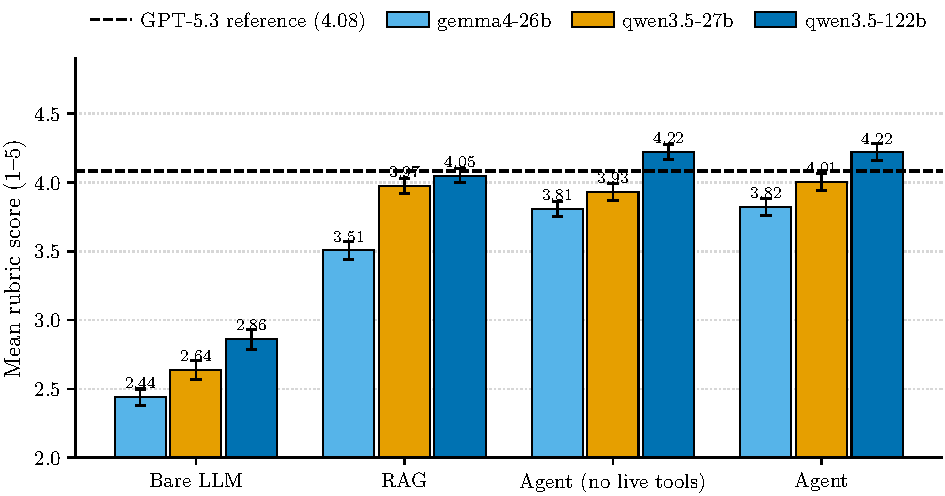
\includegraphics[width=\columnwidth]{figs/fig_headline.pdf}
\caption{The bare LLM, RAG, no-live-tools, and full agent walk
from 2.86 to 4.22 on the largest open-weight model under
\texttt{glm-5.1}; the GPT-5.3 production reference scores 4.08
on the same judge. Mean rubric score per (pipeline,
model), with $\pm 1$ standard error; each cell takes the higher
of the thinking-on/off variants.}
\label{fig:leaderboard}
\end{figure}

\paragraph{(A) An LLM alone fails on CMS-specific facts.}
The bare-LLM band sits at 2.4--2.9 across all three open-weight
models and all six question categories
(Figure~\ref{fig:by_category}). Operator questions target facts
not in pre-training: 76 factual lookups about CMS storage
elements, Rucio rules, and configuration values; 39 Jira
investigations that name specific tickets
(\texttt{CMSPROD-359}, \texttt{CMSTRANSF-1333}, \dots); 34
procedural questions about workflow recovery and resubmission.
A 122\,B model that has not seen the CMS Jira/TWiki/MonIT
corpora at training time cannot answer them; the model emits
plausible-sounding text and the judge penalises it.

\paragraph{(B) RAG closes most of the gap but is blocked on
live state.}
Adding hybrid BM25-plus-vector retrieval over the indexed CMS
TWiki and Jira (the RAG control) lifts the score to
\textbf{3.97}, recovering 1.1 of the 1.4 rubric points lost by
the bare LLM. Indexed documentation is a sufficient source for
the 144 doc-answerable questions, on which RAG averages 3.97
and the full agent 4.10 (Figure~\ref{fig:by_category}). RAG is
structurally blocked, however, on the 116 questions in the
evaluation set that require operational state: a current
transfer rate, a workflow's hourly resubmission count, a site's
readiness flag. The indexed documentation does not contain this
state, and the RAG response on such questions points the
operator to where to look rather than answering the question
directly. On the \textit{data\_query} category specifically,
RAG scores 4.07 and the full agent 4.19, but the rubric is
lenient on look-up-the-runbook responses; the qualitative gap
on live-state questions is wider than the 0.12-point lift the
rubric records.

\paragraph{(C) The agent loop closes the next 0.25 points by
composition.}
The no-live-tools ablation runs the same ReAct loop
as the full agent over the same documentation sources as RAG,
but iterates: search, fetch-by-id, cross-source synthesis. It
reaches \textbf{4.22} against RAG's 3.97 (+0.25), without
adding new tools. The lift is largest on
\textit{jira\_investigation} (4.03 vs 3.87) and
\textit{factual\_lookup} (4.58 vs 4.24): both categories
benefit from composing across multiple retrievals. The same
loop is in the deployed pipeline; the ablation isolates the
contribution of iteration from the contribution of live tools.

\paragraph{(D) Live tools earn their cost only on
data\_query.}
The full agent reaches \textbf{4.22} in aggregate, matching the
no-live-tools ablation at 4.22 because
\textit{data\_query} is 20\% of the dataset. On
\textit{data\_query} alone, live MonIT tools raise the score
from 4.00 to 4.19 (+0.19) by accessing the live counters that
the doc-only configurations cannot reach. On the three
doc-answerable categories (Factual lookup 4.58 vs 4.21;
Procedural 4.30 vs 3.88; Exploratory 4.26 vs 4.16) and on
\textit{jira\_investigation} (4.03 vs 3.70), the no-live-tools
ablation matches or beats the full agent: live calls on
questions whose answer is in the documentation correlate with
lower scores. The mechanism is dilution. Each live MonIT call
returns a JSON payload of operational state that adds hundreds
to thousands of tokens to the agent's context, and the agent
issues several such calls per question
(Section~\ref{sec:eval_costs}, Figure~\ref{fig:tool_usage}). On
a doc-answerable question the additional context crowds out the
retrieved passages that carry the answer, and the judge
penalises the more verbose, less-focused response. The deployed
pipeline keeps live tools enabled because data-query questions
are unanswerable without them; tighter tool-use instructions
that skip live calls when question type does not require them
are a natural next step (Section~\ref{sec:discussion}).

\begin{figure*}[htbp]
\centering
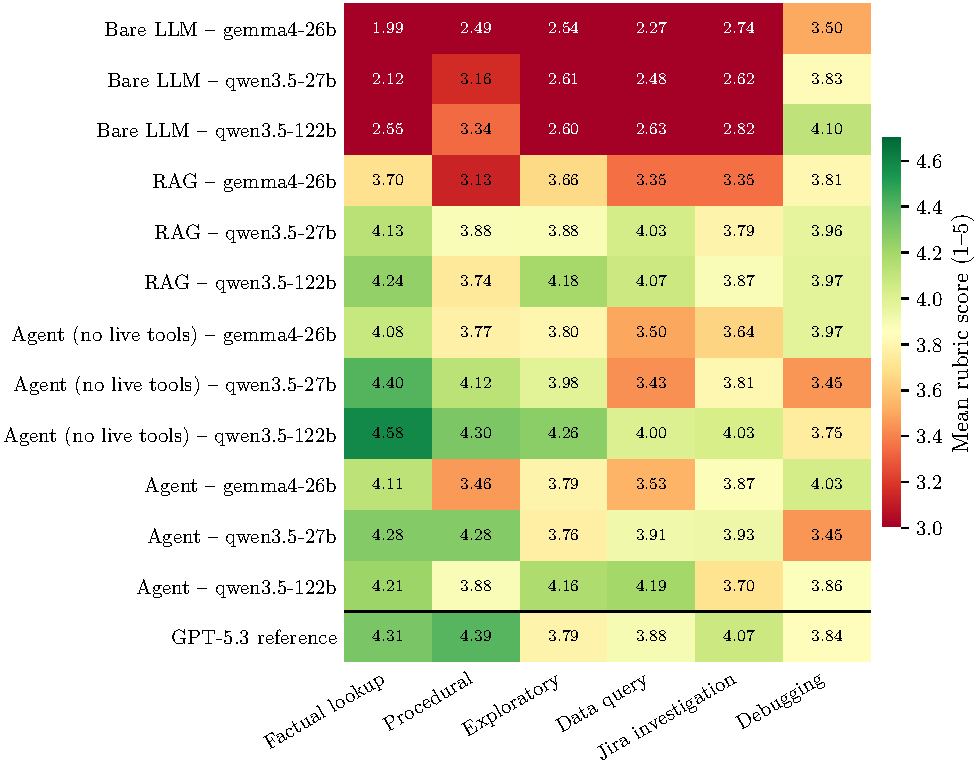
\includegraphics[width=0.82\textwidth]{figs/fig_by_category.pdf}
\caption{Live MonIT tools earn their cost on
\textit{data\_query} and lose 0.05--0.4 points on the three
doc-answerable categories. Mean rubric score per (pipeline,
model), broken down by question category; the bottom row is the
GPT-5.3 reference.}
\label{fig:by_category}
\end{figure*}

The bare-LLM, RAG, no-live-tools, and agent ordering holds on
the smaller two open-weight models as well: on
\texttt{qwen3.5-27b} the agent reaches 4.02 and on
\texttt{gemma4-26b} 3.82. On the largest open-weight model the
agent at 4.22 sits 0.14 points above the GPT-5.3 production
reference at 4.08 under the same judge.

\subsection{Two costs of the agent loop}
\label{sec:eval_costs}

The agent loop closes the gap to the production reference but
carries two measurable costs.

\paragraph{Source-faithfulness inversion.}
Figure~\ref{fig:per_dimension} reports the per-dimension scores
for the \texttt{qwen3.5-122b-a10b} configurations. On the four
core rubric dimensions the agent matches or exceeds the GPT-5.3
reference, with the largest gain on completeness ($+0.3$).
Source faithfulness inverts: the single-shot RAG control scores
\textbf{4.62}, the agent without live tools 3.71, and the full
agent 3.78. The agent's answers cite across many tool returns
rather than a single retrieval pass and score lower on
per-source attribution. The inversion replicates under the
four-judge ensemble of Section~\ref{sec:eval_ensemble}: 4.26
RAG against 3.10--3.74 for the four agents on the 53-question
subset. The same loop that buys composition trades off per-source
attribution.

\begin{figure}[htbp]
\centering
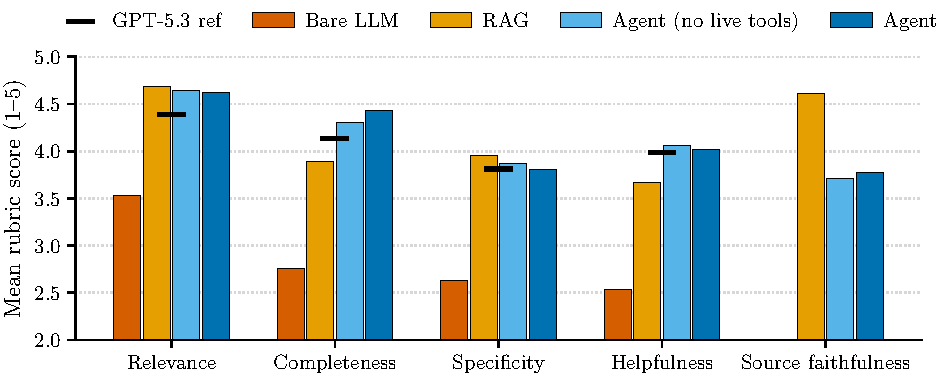
\includegraphics[width=\columnwidth]{figs/fig_per_dimension.pdf}
\caption{The agent matches the GPT-5.3 reference on the four
core dimensions but inverts under source faithfulness, where
the single-shot RAG control (4.62) leads. Per-dimension scores
on \texttt{qwen3.5-122b-a10b}; black ticks mark the GPT-5.3
reference.}
\label{fig:per_dimension}
\end{figure}

\paragraph{Quality--latency tradeoff.}
The agent with live tools runs at 60--150\,s per question on
the largest open-weight model under local Ollama; the RAG
control and the no-live-tools ablation cluster at 13--25\,s on
the same hardware. The full agent is 5--10$\times$ slower
than RAG for an additional 0.0--0.2 rubric points in aggregate.
Table~\ref{tab:runtime_53q} reports the same effect on
OpenRouter, where hosted-inference latency raises the floor.
Extended-thinking variants double the wall time without raising
scores; the deployed assistant runs the agent on the largest
model with extended thinking disabled, keeping operator-facing
latency below 90\,s.

Figure~\ref{fig:tool_usage} shows the agent's tool-call profile
by question category. On \textit{data\_query} the agent issues
5.4 HTCondor MonIT calls per question against 2.3 documentation
calls; on every other category it falls back to documentation
retrieval. The agent self-routes, which is one half of the
routing argument in Section~\ref{sec:discussion}.

\begin{figure}[htbp]
\centering
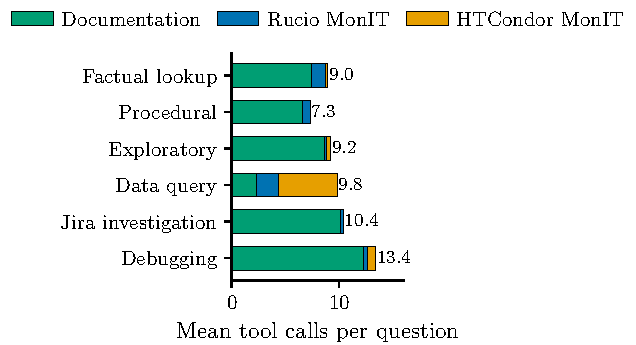
\includegraphics[width=\columnwidth]{figs/fig_tool_usage.pdf}
\caption{The agent routes by question type: HTCondor MonIT
dominates on \textit{data\_query}; every other category falls
back to documentation retrieval. Mean tool calls per question
by category, agent on \texttt{qwen3.5-122b-a10b}.}
\label{fig:tool_usage}
\end{figure}

\subsection{The four-step ordering survives a four-judge ensemble}
\label{sec:eval_ensemble}

Four LLM judges from independent providers rate every response
on the 53-question subset under the rubric of
Section~\ref{sec:eval_methodology}: \texttt{glm-5.1}
\cite{glm130b}, \texttt{gemini-3.1-pro-preview},
\texttt{gpt-5.5-2026-04-23} (rating its own family), and
\texttt{claude-opus-4.7}. All four judges score the 265
(configuration, question) tuples.

Every judge places the closed-frontier \texttt{gpt-5.5}
agent first and the \texttt{qwen3.6-27b} RAG control last
(Table~\ref{tab:judge_ensemble_per_config}). The pipeline
ordering of Section~\ref{sec:eval_lifts} survives a judge swap
on the one configuration shared across both tracks
(\texttt{qwen3.5-122b-a10b} agent) and across four further
configurations the local cluster could not host.

\begin{table*}[htbp]
\centering
\caption{Per-judge per-configuration mean rubric score on the
53-question subset (average of the four core dimensions; 1--5
scale). Every judge places the production-class
\texttt{gpt-5.5} agent first and the \texttt{qwen3.6-27b} RAG
control last.}
\label{tab:judge_ensemble_per_config}
\begin{tabular}{lccccc}
\toprule
\textbf{Configuration} & \textbf{glm-5.1} & \textbf{gemini-3.1-pro} & \textbf{gpt-5.5} & \textbf{opus-4.7} & \textbf{Ensemble} \\
\midrule
\texttt{gpt-5.5-2026-04-23} agent & 4.83 & 4.88 & 4.09 & 4.72 & \textbf{4.63} \\
\texttt{qwen3.6-27b} agent        & 4.56 & 4.83 & 3.71 & 4.49 & \textbf{4.40} \\
\texttt{qwen3.5-122b-a10b} agent  & 4.48 & 4.78 & 3.53 & 4.32 & \textbf{4.28} \\
\texttt{qwen3.6-35b-a3b} agent    & 4.48 & 4.55 & 3.52 & 4.33 & \textbf{4.22} \\
\texttt{qwen3.6-27b} RAG          & 3.95 & 4.41 & 3.26 & 3.50 & \textbf{3.78} \\
\bottomrule
\end{tabular}
\end{table*}

The per-dimension ensemble means
(Table~\ref{tab:judge_ensemble_per_dim}) replicate the
source-faithfulness inversion of
Section~\ref{sec:eval_costs}: the \texttt{qwen3.6-27b} RAG
control scores 4.26 on source faithfulness against 3.10--3.74
for the four agents, while losing 0.5--1.2 points to the
closed-frontier \texttt{gpt-5.5} agent on every other dimension. The
\texttt{gpt-5.5} agent leads on every dimension except source
faithfulness; the open-weight agent ordering is stable across
the four core dimensions.

\begin{table*}[htbp]
\centering
\caption{Per-dimension ensemble-mean rubric score on the
53-question subset (1--5 scale), averaged across the four
judges of Table~\ref{tab:judge_ensemble_per_config}. Source
faithfulness inverts between the agent and RAG pipelines,
matching the 260-question single-judge result of
Section~\ref{sec:eval_costs}.}
\label{tab:judge_ensemble_per_dim}
\begin{tabular}{lccccc}
\toprule
\textbf{Configuration} & \textbf{Relevance} & \textbf{Completeness} & \textbf{Specificity} & \textbf{Helpfulness} & \textbf{Src.\ faith.} \\
\midrule
\texttt{gpt-5.5-2026-04-23} agent & \textbf{4.99} & \textbf{4.79} & \textbf{4.19} & \textbf{4.56} & 3.74 \\
\texttt{qwen3.6-27b} agent        & 4.86 & 4.53 & 3.92 & 4.27 & 3.46 \\
\texttt{qwen3.5-122b-a10b} agent  & 4.82 & 4.48 & 3.72 & 4.10 & 3.25 \\
\texttt{qwen3.6-35b-a3b} agent    & 4.77 & 4.47 & 3.64 & 4.01 & 3.10 \\
\texttt{qwen3.6-27b} RAG          & 4.53 & 3.62 & 3.44 & 3.53 & \textbf{4.26} \\
\bottomrule
\end{tabular}
\end{table*}

One judge-protocol caveat: \texttt{gpt-5.5-2026-04-23} as a
judge is the harshest of the four (4.09 on its own family's
response against the 4.63 ensemble mean) and concentrates that
harshness on the specificity dimension (2.56 against an ensemble
mean of 3.78). The ensemble ordering reported above
de-emphasises this single-judge offset.

\subsection{Human evaluation on the 53-question subset}
\label{sec:eval_human_53}

LLM judges carry length~\cite{hu2025lengthbias},
position~\cite{wang2023fair}, and
self-preference~\cite{panickssery2024selfpref} biases.
A panel of five CMS Computing Operations domain experts grades
the 53-question subset across the five configurations, blind to
configuration, providing a non-LLM reference against which the
judge scores in Sections~\ref{sec:eval_lifts}--\ref{sec:eval_ensemble}
can be checked. The grading round opened on 2026-05-11; results
are reported once the panel completes the round.

The 53 questions are selected by an experienced CompOps operator
from the 260-question curated set of
Section~\ref{sec:question_patterns} and split across
24~factual-lookup, 19~procedural, 5~Jira-investigation,
4~exploratory, and 1~debugging question.
For each question, the five responses are randomly relabeled
A--E with a per-question permutation; the mapping from label to
configuration is hidden from the annotators and stored in a
sidecar. Each response is scored on two 1--5 dimensions:
\emph{correctness} (factual accuracy against operator practice
and the cited sources) and \emph{usefulness} (whether an
on-call operator can act on the response without further
investigation). The annotators also rank A--E from best to
worst, with ties allowed.

The grading platform is Argilla 2.8~\cite{argilla}, deployed on
a CMS-internal node and fronted by an oauth2-proxy GitHub
allowlist. The task-distribution setting requires at least two
submissions per record, so every record carries two or more
independent ratings. Retrieved sources appear as a
metadata-only collapsible block of clickable links (Jira ticket,
TWiki page, GitHub document) rather than as raw retrieved text.

Three quantities are reported once grading completes.
Per-configuration means on correctness and usefulness over the
53 questions place each configuration on the same scale
(Table~\ref{tab:human_eval_per_config}).
Inter-annotator agreement is reported as the mean pairwise
Pearson on the continuous dimensions and mean pairwise
Kendall's~$\tau$ on the rankings, with $r = \textbf{[TBD]}$
and $\tau = \textbf{[TBD]}$. The consistency between the
human ranking and the judge-ensemble ranking from
Section~\ref{sec:eval_ensemble} across the five configurations
is reported as a rank correlation ($\tau = \textbf{[TBD]}$),
bounding how much of the LLM-judge ordering survives under
human scrutiny.

\begin{table*}[htbp]
\centering
\caption{Per-configuration human-evaluation results on the
53-question subset, averaged across the annotator panel.
Correctness and usefulness are 1--5 means; rank is the mean
A--E ranking position (1 = best). Values pending the close of
the grading round.}
\label{tab:human_eval_per_config}
\begin{tabular}{lccc}
\toprule
\textbf{Configuration} & \textbf{Correctness} & \textbf{Usefulness} & \textbf{Mean rank} \\
\midrule
\texttt{gpt-5.5-2026-04-23} agent & \textbf{[TBD]} & \textbf{[TBD]} & \textbf{[TBD]} \\
\texttt{qwen3.5-122b-a10b} agent  & \textbf{[TBD]} & \textbf{[TBD]} & \textbf{[TBD]} \\
\texttt{qwen3.6-35b-a3b} agent    & \textbf{[TBD]} & \textbf{[TBD]} & \textbf{[TBD]} \\
\texttt{qwen3.6-27b} agent        & \textbf{[TBD]} & \textbf{[TBD]} & \textbf{[TBD]} \\
\texttt{qwen3.6-27b} RAG          & \textbf{[TBD]} & \textbf{[TBD]} & \textbf{[TBD]} \\
\bottomrule
\end{tabular}
\end{table*}
